%%%%%%%%%%%%%%%%%%%%%%%%%%%%%%%%%%%%%%%%%%%%%%%%%%%%%%%%%%%%%%%%%%%%%%%%
% Plantilla TFG/TFM
% Escuela Politécnica Superior de la Universidad de Alicante
% Realizado por: Jose Manuel Requena Plens
% Contacto: info@jmrplens.com / Telegram:@jmrplens
%%%%%%%%%%%%%%%%%%%%%%%%%%%%%%%%%%%%%%%%%%%%%%%%%%%%%%%%%%%%%%%%%%%%%%%%
\chapter{Introduction}\label{chap:introduction}

This chapter sets the stage for the scope of this project. It provides a brief
summary of the issue in question, proceeds with an extensive discourse on the
project's inspiration, and finally, presents an overview of the chapters that
follow in this document.

\section{Motivation and Context}

Addressing the global challenge of obesity, which affects a considerable
proportion of the population, is a matter of public health concern. Having
experienced the struggles of obesity first-hand, I am deeply committed to
addressing this issue. It is my belief that our society can greatly benefit
from reducing the impact of obesity, ultimately enhancing the quality of life
for countless individuals. This project aims to contribute towards achieving
this goal.

Tech4Diet is a research initiative that investigates the morphological changes
induced by obesity treatments in the human body. The project has been supported
by the \textit{Agencia Estatal de Investigación} and the \textit{Fondo Europeo
	de Desarrollo Regional} (FEDER), under the leadership of Jorge Azorín López.

In an earlier venture, Tech4Diet developed a system that enabled patients
undergoing weight loss treatment to visualize their body's 3D scans throughout
their journey (reference required). The patient's body is captured during the
treatment using an RGB-D camera, more specifically the Intel RealSense D435.
This 3D model of the human body is presented to the patient during various
sessions through a virtual reality headset. This innovative method was
conceived to strengthen motivation and increase adherence to the treatment
program.

\begin{figure}
	\centering
	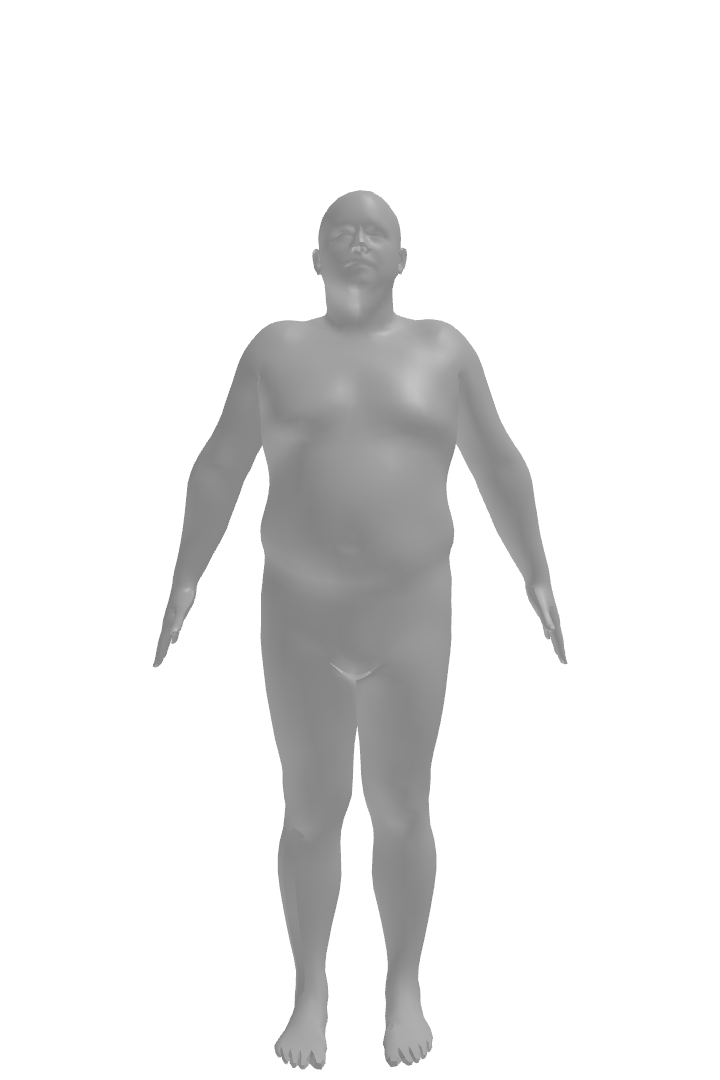
\includegraphics[width=75pt]{files/patients/8_2}
	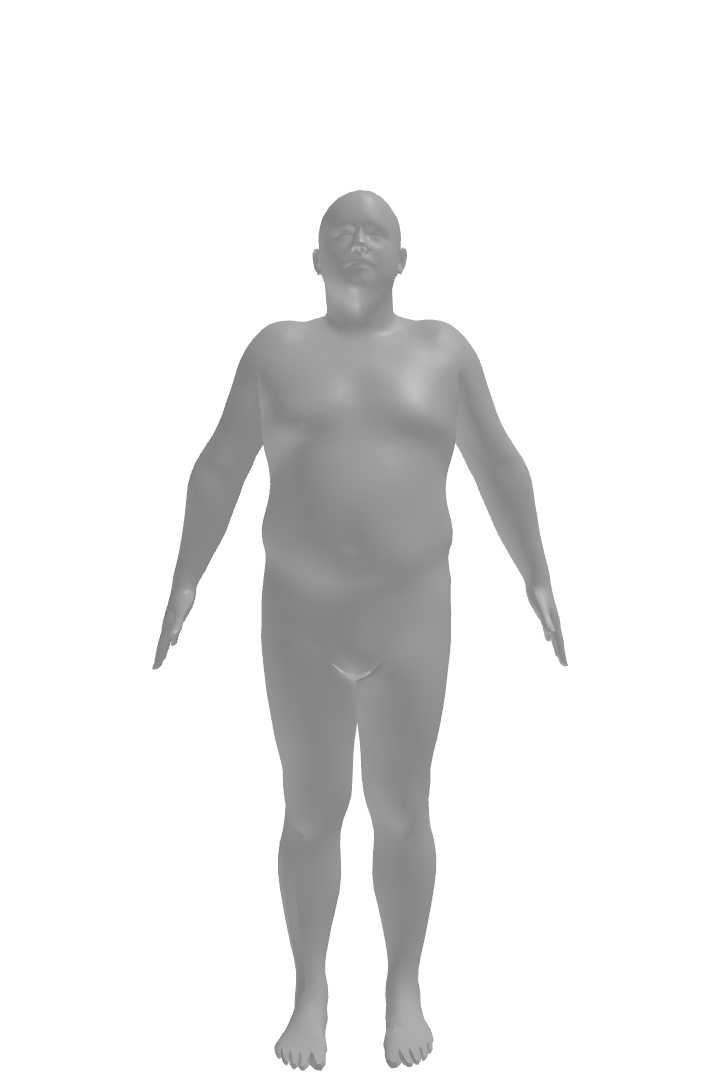
\includegraphics[width=75pt]{files/patients/8_3}
	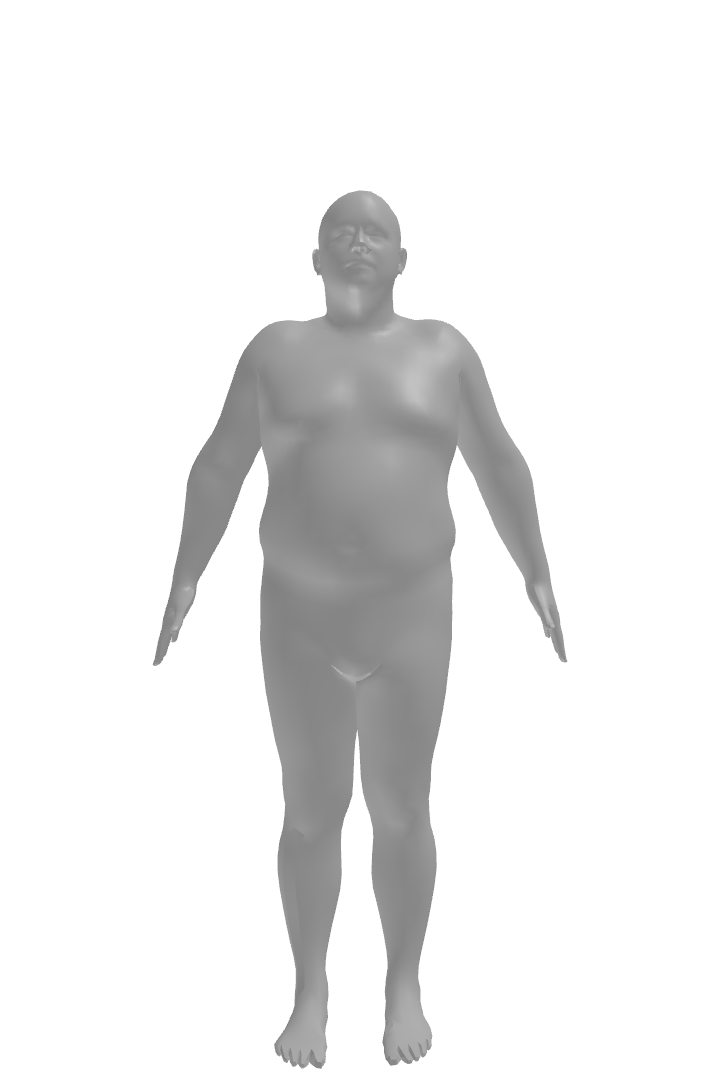
\includegraphics[width=75pt]{files/patients/8_4}
	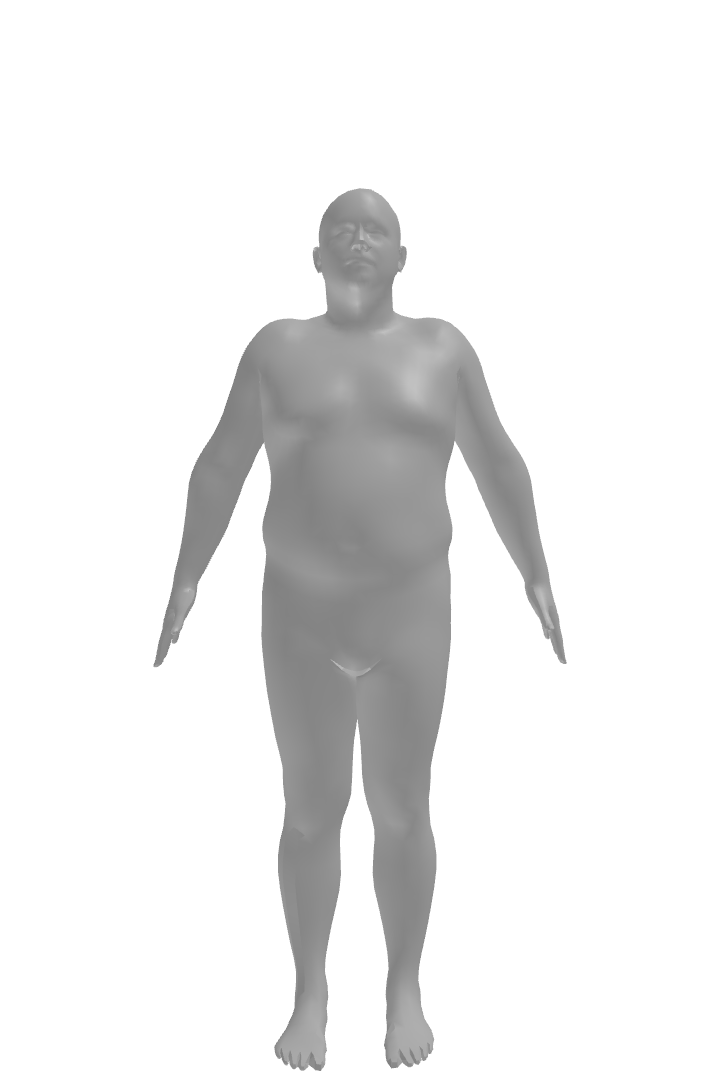
\includegraphics[width=75pt]{files/patients/8_5}
	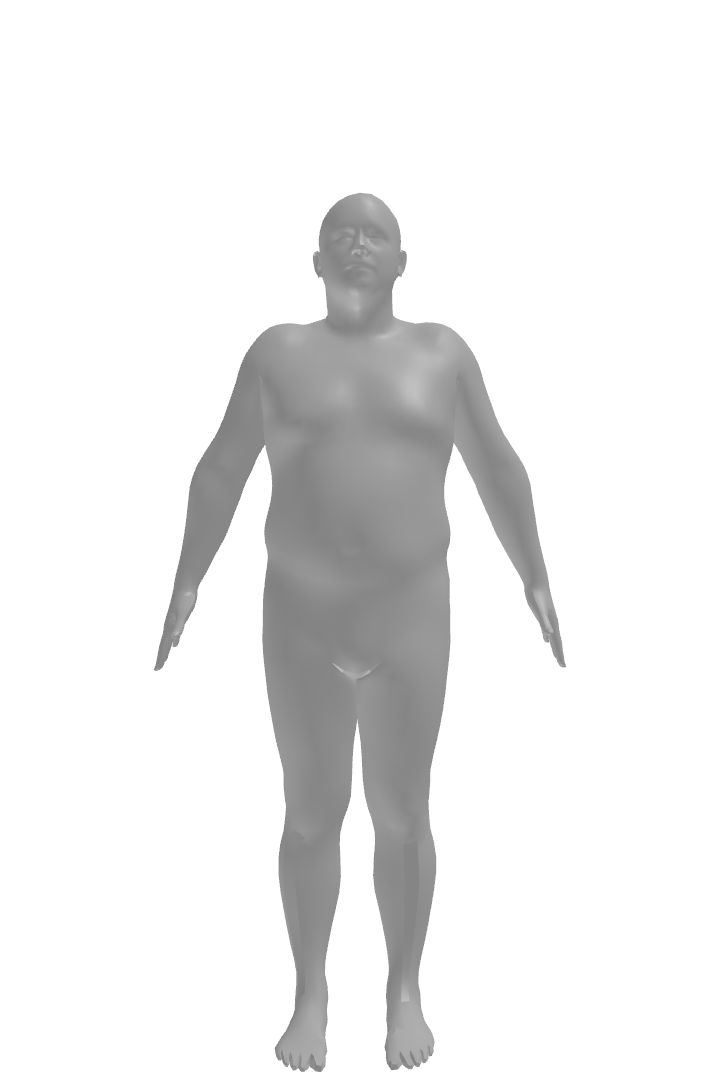
\includegraphics[width=75pt]{files/patients/8_6}
	\caption[Reconstructed 3D body of a patient's scans]{3D model reconstruction of a patient's body at different stages of a weight loss
		treatment. Each scan is taken approximately a month apart, with a total
		weight loss of 3.8 kg.}
\end{figure}

Apart from body scans, the study also collated other medical data, including
variables such as weight, localized fat and muscle mass, activity levels, and
psychological factors.

Building on this, we sought to explore the feasibility of using the datasets
acquired from this prior study to develop a predictive model. The intention was
for this model to forecast changes in a person's body undergoing weight loss
treatment before the treatment concludes, thereby bolstering adherence to the
treatment regimen.

The present work encapsulates the development of such a model. This encompasses
analyzing data from the earlier study, examining existing techniques in human
body model representation, encoding patient data using the selected
representation, designing a neural network architecture for predicting patient
body changes, training, and evaluating the model. Ultimately, the model
generates 3D meshes of the predicted body changes.

The following chapters will delve deeper into the specifics of this process.
Chapter \ref{chap:data} examines the data collected during the previous study
and explains how we prepared it for use in our model. It also delineates the
encoding process of the human body scans. Chapter \ref{chap:nn} explores the
neural network architecture we constructed for this project, including the
training process and the results we obtained. Chapter \ref{chap:results}
interprets the outcomes of our model, and chapter \ref{chap:conclusion}
concludes the document by recapping the work done and suggesting potential
future research directions.

\section{State of the Art}\label{sec:sota}

In this section, we provide a comprehensive overview of the \gls{sota}
methodologies for human body representation, as well as a first overview of
generative neural networks suitable for our purpose. The knowledge derived from
these studies in human body representation paved the way for a submission to
the \gls{iwann} 2023 conference. \todo{link}

\subsection{3D Human Body Representation}

Advancements in 3D human body recovery have largely been driven by the
development of parametric models. These models use sets of parameters to
represent body shape and pose, becoming instrumental in the reconstruction of
3D human bodies. They vary in focus—some emphasize body deformations, others
shape and pose optimization, while others separate body shape into
identity-specific and pose-dependent components. Each approach has its own
advantages and applications, contributing to improved accuracy and stability in
representing human body shapes and poses.

Broadly speaking, human body representations can be categorized based on the
required input type and the resulting output:

\subsubsection{Input-Output Typology}

Taxonomy of models according to their input:

\begin{itemize}
	\item \textbf{2D input:} Models that utilize 2D images or videos as input.
	\item \textbf{3D input:} Models that require 3D point clouds as input data.
	\item \textbf{Parametric models:} Models that require a set of parameters describing the body.
\end{itemize}

We can also categorize models based on their output:

\begin{itemize}
	\item \textbf{2D space:} These models output human bodies in 2D pixel space, such as images or videos.
	\item \textbf{3D meshes:} Models that generate a 3D mesh of the body.
	\item \textbf{3D voxel:} Models that produce a 3D voxel grid of the body.
	\item \textbf{\gls{nerf}:} Models that render the object directly from a specific viewpoint.
\end{itemize}

\subsubsection{Generation of 3D Human Body Models}

In the realm of 3D human model generation, two primary approaches exist. One
uses a general-purpose generator system guided to generate human models. The
second deploys a generator specifically designed for creating human models from
the beginning.

Human-specific generators have gained considerable attention in recent years,
with several notable examples:

\begin{itemize}
	\item \textbf{SiCloPe} \citep{DBLP:journals/corr/abs-1901-00049} models clothed human bodies using deep generative models.
	\item \textbf{PIFu} and \textbf{PIFuHD} \citep{pifu, pifuhd} are effective implicit representations aligning 2D image pixels with their corresponding 3D object.
	\item \textbf{Tex2Shape} \citep{alldieck2019tex2shape} infers detailed full human body shape from a single photograph.
	\item \textbf{HumanMeshNet} \citep{DBLP:journals/corr/abs-1908-06544} and \textbf{DeepHuman} \citep{DBLP:journals/corr/abs-1903-06473} focus on 3D human body reconstruction from a monocular image.
	\item \textbf{HumanGen} \citep{jiang2022humangen} provides a detailed 360° realistic free-view rendering of the human body.
	\item \textbf{HumanNeRF} \citep{weng_humannerf_2022_cvpr} offers a high-fidelity free-view synthesis of dynamic humans.
\end{itemize}

For general-purpose generators, \textbf{CoCosNet} and its second version
\citep{CoCosNet, CoCosNet2} have shown significant effectiveness in
cross-domain image translation.

\subsubsection{Parametric Models}

Parametric models for representing and generating 3D human body shapes and
poses have gained significant interest in recent years. These models are based
on adjustable parameters that allow for pose and shape modifications, enabling
the reconstruction and creation of unique human bodies. They find applications
in animation, virtual reality, and garment simulation.

One notable early work in this field is Allen's method \citep{allen:2003},
which utilizes a statistical model to create a parametric model of the human
body. It matches the pose of a human in a 3D scan by interpolating from example
scans with similar joint angles. However, it does not account for how body
shape changes with pose, primarily serving as a hole-filling technique.

Another significant model is SCAPE \citep{scape}, which represents body
deformations caused by shape and pose as triangle deformations. It uses linear
regression to determine pose deformations. Although it aims to represent muscle
deformations, it lacks specificity for different muscle activities and fails to
capture motion-related tissue perturbations.

BlendSCAPE \citep{blendscape} extends the SCAPE model by optimizing shape and
pose registration simultaneously using a blending technique. However, its
formulation is incompatible with standard graphics packages and may not be
suitable for common graphics applications.

SymmetricSCAPE \citep{CHEN201952}, a variant of SCAPE and BlendSCAPE,
incorporates symmetry constraints to enhance the accuracy and stability of the
model, resulting in a more robust representation of the 3D human body.

The \gls{smpl} \citep{SMPL:2015} model is widely used for 3D human body shape
and pose representation. It separates body shape and pose into parameters and
employs a vertex-based skinning approach with corrective blend shapes, offering
greater flexibility. It is compatible with various graphics applications.

Improvements to the \gls{smpl} model include SMPL-H, which incorporates
articulated hand pose and shape parameters, and SMPL-X, which includes hand and
face pose and shape parameters \citep{SMPL-X:2019}

The STAR model \citep{STAR:2020} addresses limitations of \gls{smpl}, such as
reducing mesh volume around joints, by learning corrective blend shapes. It
offers realistic deformations of the 3D human body while requiring fewer
parameters than \gls{smpl}.

Another approach is presented in BLSM \citep{doi:10.1007/978-3-030-58558-7_1},
which utilizes a bone-level skinning method. It establishes the skeleton first
by determining bone lengths and angles, incorporating identity-specific
variations, and then applies linear blend skinning for animation.

\subsection{Neural Networks}

Neural networks, more formally known as artificial neural networks, are a
subset of machine learning models inspired by biological brain systems. These
computational models mimic the neurons' interconnections and behavior in a
biological brain, which is how they derive the name `neural networks'.

At the core of a neural network is the concept of a `neuron' or `node'. These
neurons are organized into layers: the input layer, one or more hidden layers,
and the output layer. Each neuron within these layers is interconnected with
neurons from the subsequent layer. Figure \ref{fig:nn} shows a neural network
with three input neurons, four hidden neurons, and two output neurons.

\textbf{Input layer:} This layer receives raw input signals,
analogous to sensory data in a biological system.

\textbf{Hidden layers:} These layers perform computations and transformations
on the data from the previous layer. The complexity of the model increases with
the number of hidden layers and neurons in each layer.

\textbf{Output layer:} The final layer translates the outcomes of the hidden
layers into the format relevant to the task at hand, be it classification,
regression, or something else.

\begin{figure}
	\centering
	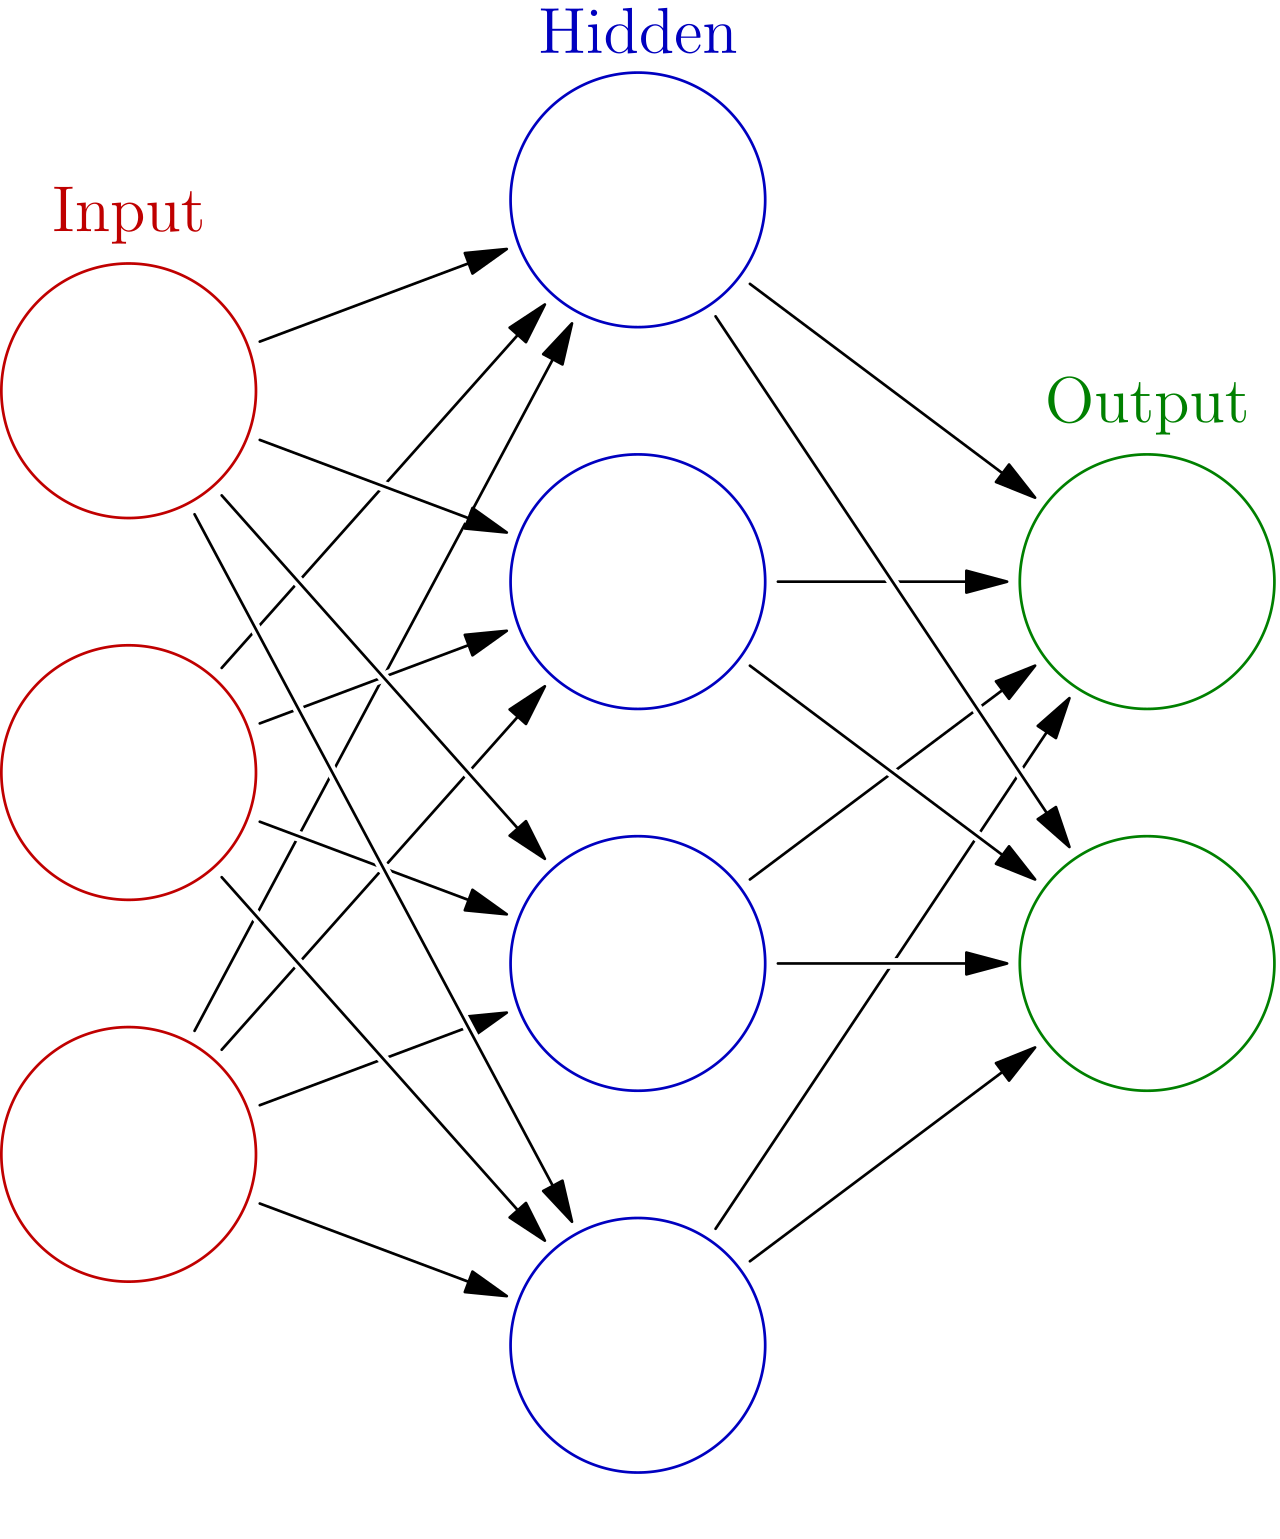
\includegraphics[width=0.3\textwidth]{files/nn.png}
	\caption{A simple neural network \citep{glosserca}.}
	\label{fig:nn}
\end{figure}

Each connection between the neurons has an associated `weight', which impacts
the input's influence on the output. During the training process, these weights
are adjusted to minimize the difference between the predicted output and the
actual output.

Neural networks learn from data using a process called backpropagation, an
algorithm that calculates the gradient of the loss function (a measure of the
network's error) with respect to the weights. This gradient is then used to
update the weights, typically via an optimization algorithm like \gls{sgd}.

These fundamental aspects of neural networks make them incredibly flexible and
powerful. They are capable of learning complex patterns and relationships in
data, and can be applied to a wide range of tasks such as image and speech
recognition, natural language processing, medical diagnosis, financial
forecasting, and much more.

There are various types of neural networks, each designed for specific tasks or
to work with specific types of data. Examples include \glspl{cnn} for image and
video processing, \glspl{rnn} for sequential data, and \glspl{gan} for
generating new data that resembles the input data. Each of these networks
builds on the basic principles outlined above but includes additional
structures or processes to better handle their specific tasks.

\subsection{Neural Networks for Sequential Data}

In Chapter \ref{chap:nn}, we will examine different types of networks that are
specialized for handling sequential or temporal data. We'll start with a look
at \glspl{rnn} \citep{doi:10.1073/pnas.79.8.2554}, which are known for their
ability to handle sequences due to their `memory' features.

Next, we'll be discussing \glspl{lstm} and \glspl{gru}
\citep{lstm:1997,gru:2014}, both of which are variants of \glspl{rnn}. While
\glspl{lstm} introduce concepts such as a cell state and gates to control
information flow, \glspl{gru} take a simpler yet equally effective approach.

We will also provide insights on Transformer Networks \citep{attention:2017}, a
more recent advancement in the field of Neural Networks. These are quite
different from \glspl{rnn}. Instead of relying on recurrent processing,
Transformers use an attention mechanism that can process entire sequences of
data at once, which helps them understand dependencies in data more
effectively.

After this analysis, we will select the most promising architecture, implement
it using a neural network framework, train it on our data, and evaluate its
performance. This will be covered in Chapter \ref{chap:nn}.

\section{Objectives}\label{objectives}

This project is guided by the following objectives. They are designed to
provide a clear structure for the work and ensure that the project's goals are
achieved, as well as serving for the author to develop a deeper understanding
of the subject matter.

\begin{itemize}
	\item \textbf{Objective 1: Comprehensive Literature Review}
	      \begin{itemize}
		      \item Understand the current state of the art in human body representation and
		            generation.
		      \item Critically analyze the advantages and disadvantages of existing methodologies.
		      \item Identify the most promising approach to guide our project.
	      \end{itemize}

	\item \textbf{Objective 2: Data Preparation}
	      \begin{itemize}
		      \item Conduct a thorough exploration of the project's data and understand its
		            characteristics.
		      \item Implement rigorous preprocessing steps to ensure the data's quality and
		            consistency.
		      \item Investigate potential data augmentation techniques to enhance the robustness of
		            our models.
	      \end{itemize}

	\item \textbf{Objective 3: Neural Network Development}
	      \begin{itemize}
		      \item Survey potential neural network architectures suitable for time series
		            prediction problems.
		      \item Design a bespoke neural network architecture that is optimized for future human
		            body shape generation.
		      \item Implement and train the proposed neural network, fine-tuning its parameters for
		            optimal performance.
		      \item Evaluate the predictive performance of our trained network.
	      \end{itemize}

	\item \textbf{Objective 4: Result Evaluation}
	      \begin{itemize}
		      \item Generate human body shape predictions using our past data.
		      \item Conduct an evaluation of our model's predictive performance, discussing its
		            potential applications and limitations.
	      \end{itemize}

\end{itemize}
